\subsubsection{Testbench và Kết quả mô phỏng Instruction Register (IR)}

\textbf{a. Mô tả Testbench} \\
\begin{itemize}
    \item Kiểm tra đồng bộ: Kích hoạt \texttt{rst} để đảm bảo
    \texttt{opcode} và \texttt{addr} được đưa về giá trị 0 tại cạnh lên của xung clock.
    \item Kiểm tra giải mã: Nạp các dữ liệu 32-bit khác nhau để xác nhận các bit cao (31-29) được tách vào \texttt{opcode} 
    và các bit thấp (28-0) được tách vào \texttt{addr}.
    \item Kiểm tra đường truyền dữ liệu: Thay đổi ngõ vào \texttt{data\_in} khi tín hiệu \texttt{ld\_ir} ở mức thấp để 
    chứng minh dữ liệu cũ vẫn được duy trì.
\end{itemize}

\textbf{b. Mã nguồn Testbench}
\begin{lstlisting}[language=Verilog, caption={Testbench Instruction Register}]
`timescale 1ns / 1ps

module tb_instruction_reg();

    reg          clk;
    reg          rst;
    reg          ld_ir;
    reg  [31:0] data_in;
    
    wire [2:0]  opcode;
    wire [28:0] addr;

    instruction_reg uut (
        .clk(clk),
        .rst(rst),
        .ld_ir(ld_ir),
        .data_in(data_in),
        .opcode(opcode),
        .addr(addr)
    );

    always #5 clk = ~clk;

    initial begin
        clk = 0; rst = 0; ld_ir = 0; data_in = 32'b0;

        $display("----------");
        $display(" Time|rst|ld_ir|Data_in|Opcode|Address");
        $display("----------");
        $monitor("%10t|%b|%b|%h|%b|%h", 
                 $time, rst, ld_ir, data_in, opcode, addr);

        //Kiem tra Reset dong bo
        #12; rst = 1;
        #10; rst = 0;

        //Thu nap lenh ADD (010) voi dia chi 0x00000FF
        #10; 
        data_in = {3'b010, 29'h00000FF}; 
        ld_ir = 1; // Cho phep nap
        #10;
        ld_ir = 0; // Khoa nap

        //Thay doi data_in nhung ld_ir = 0 (Gia tri cu phai giu nguyen)
        #10;
        data_in = {3'b111, 29'hFFFFFFF}; 
        #10;

        //Nap lenh moi JMP (111)
        #10;
        ld_ir = 1;
        #10;
        ld_ir = 0;

        // Reset giua chung
        #10;
        rst = 1;
        #10;
        rst = 0;

        #20;
        $display("----------");
        $display("Hoan thanh mo phong Instruction Register!");
        $finish;
    end
endmodule
\end{lstlisting}

\textbf{c. Sơ đồ mạch RTL} 
\begin{figure}[H]
    \centering
   
    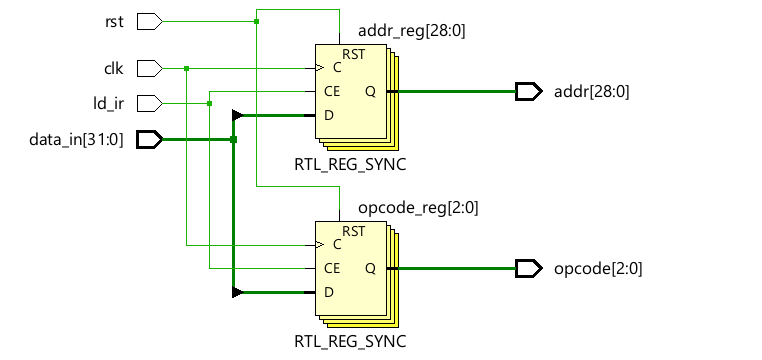
\includegraphics[width=0.7\textwidth]{sodoIR.png} 
    \caption{Sơ đồ mạch RTL của khối Instruction Register}
    \label{fig:ir_rtl}
\end{figure}

\textbf{d. Kết quả xuất ra màn hình} 

\begin{figure}[H]
    \centering
    % Thay 'ir_console.png' bang ten file anh console cua ban
    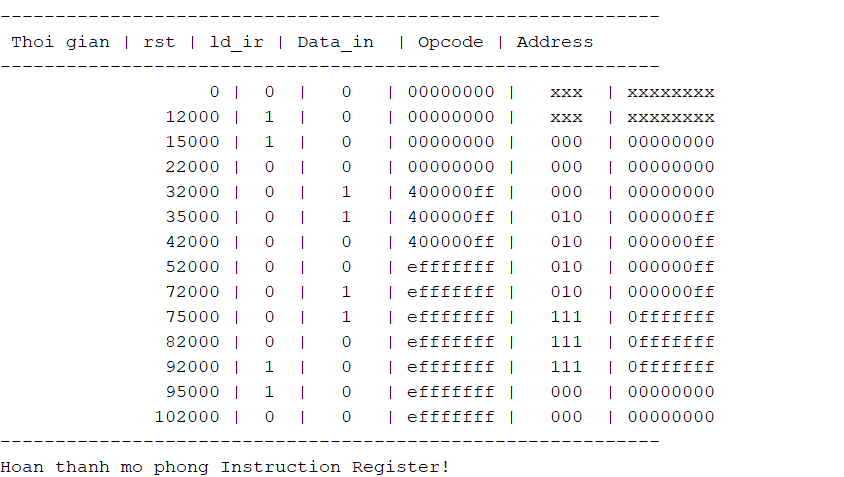
\includegraphics[width=0.8\textwidth]{consoleIR.png} 
    \caption{Kết quả chạy Testbench Instruction Register trên Console}
    \label{fig:ir_console}
\end{figure}

Dựa trên log mô phỏng, khi tín hiệu \texttt{ld\_ir} được kích hoạt, 
giá trị \texttt{opcode} và \texttt{addr} ngay lập tức cập nhật dựa trên 3 bit cao và 29 bit thấp của \texttt{data\_in}.
 Tại các thời điểm \texttt{ld\_ir} bằng 0, dù \texttt{data\_in} có biến động, 
 các giá trị ngõ ra vẫn giữ nguyên.

\textbf{e. Giản đồ sóng} 

\begin{figure}[H]
    \centering
    % Thay 'ir_waveform.png' bang ten file anh waveform cua ban
    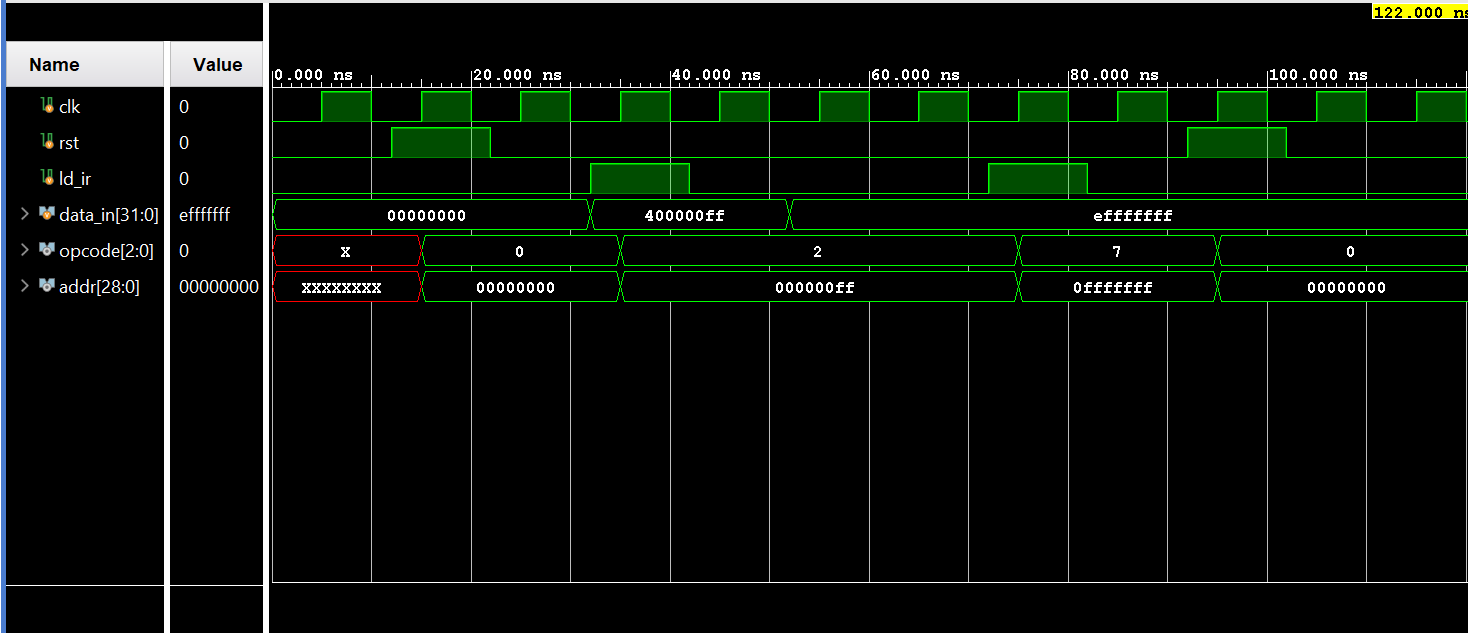
\includegraphics[width=\textwidth]{waveIR.png} 
    \caption{Giản đồ sóng mô phỏng khối Instruction Register}
    \label{fig:ir_waveform}
\end{figure}

